\chapter{ECG prediction using a Recurrent Neural Network}\label{ch:rnn}

In this chapter I will discuss the design and implementation of a Long
Short-Term Memory (LSTM) Recurrent Neural Network (RNN) that is able to predict
the next value of the ECG signal given as input the ECG signal up to the
previous time step and some other signals. This implements the requirements for
the Task 4.2 of the Project Specifications.

The approach followed to develop the RNN is similar to the one used in
\chref{ch:rnn}. In particular, since training of CNNs and RNNs is similar, the
script \code{rnntrain.m} is a copy-pasted and adapted version of the
\code{cnntrain.m} script.

Note that, for this task, I've changed again the way data augmentation is
performed. Here, I'll extract a total of \(60000\) samples of \(61\) time
steps, since \(6000\) samples were not sufficient to train the RNN. Moreover,
the \code{fixdata} stage is instructed to divide samples whenever a hole larger
than 2 milliseconds (the fastest sampling rate) is found in the data: to train
an RNN, I do not want to have any hole at all in the data.

The developed RNN uses 8 signals of the 11 signals available in the dataset.
The 8 signals selected are all the signals that are sampled with a sampling
rate of \(500\) Hz (the \code{pleth\_*} signals, the \code{temp\_3} signal
and, obiously, the \code{ecg} signal). This choice has been made in order to
avoid to use signals sampled at lower rates, which remain constants for some
time steps and may degrade the performance of the network.

\section{Selection of the size of the window}\label{sec:rnnwinsize}

The starting LSTM RNN architecture is shown in \lstref{lst:startingrnn}.

\lstinputlisting[language={matlab}, label={lst:startingrnn},
style={Matlab-editor}, basicstyle={\footnotesize\ttfamily}, caption={Starting
architecture for the LSTM.}]{startingrnn.m}

RNN definitions from 1 to 10 are used to find the optimal window size, using
\(50\) as the number of neurons and training for \(50\) epochs. Results are
shown in \tableref{table:rnnwinsize}. A window size of \(10\) is a valid
choice, based on the RMSE on the best loss iteration.

\begin{table}[hbtp]
	\centering
	\begin{tabular}{|c|c|c|c|}
		\toprule
		\# & Window size & RMSE & Best RMSE \\
		\midrule
		1 & 10 & \(6128.04\) & \(3087.69\) \\
		2 & 20 & \(8666.25\) & \(8949.86\) \\
		3 & 30 & \(4839.1\) & \(5496.51\) \\
		4 & 40 & \(7023.05\) & \(5328.75\) \\
		5 & 50 & \(7434.16\) & \(6413.42\) \\
		6 & 60 & \(9297.86\) & \(8541.49\) \\
		7 & 12 & \(5614.25\) & \(5315.68\) \\
		8 & 15 & \(7863.83\) & \(6274.77\) \\
		9 & 9 & \(7406.52\) & \(4481.75\) \\
		10 & 8 & \(8528.44\) & \(6514.86\) \\
		\bottomrule
	\end{tabular}
	\caption{Trying different window sizes for the
	RNN.}\label{table:rnnwinsize}
\end{table}

\section{Selection of the normalization algorithm}\label{sec:rnnnormalization}

I've tried all possible choices for the normalization algorithm for the input
sequences. Results in \tableref{table:rnnnormalization}.

\begin{table}[hbtp]
	\centering
	\begin{tabular}{|c|c|c|c|}
		\toprule
		\# & Normalization algorithm & RMSE & Best RMSE \\
		\midrule
		1 & \code{rescale-symmetric} & \(6128.04\) & \(3087.69\) \\
		11 & \code{zerocenter} & \(13938.16\) & \(11285.47\) \\
		12 & \code{zscore} & \(3157.22\) & \(2930.36\) \\
		13 & \code{rescale-zero-one} & \(10997.16\) & \(10982.06\) \\
		\bottomrule
	\end{tabular}
	\caption{Changing the normalization algorithm for the
	RNN.}\label{table:rnnnormalization}
\end{table}

Best results were obtained using \code{zscore}.

\section{Selection of the number of neurons}\label{sec:rnnneurons}

RNN definitions from 14 to 20 are used to try different values for the number
of neurons in the LSTM layer. Results are shown in \tableref{table:rnnneurons}.
Best results are obtained using \(65\) neurons.

\begin{table}[hbtp]
	\centering
	\begin{tabular}{|c|c|c|c|}
		\toprule
		\# & \# of neurons & RMSE & Best RMSE \\
		\midrule
		12 & 50 & \(3157.22\) & \(2930.36\) \\
		14 & 20 & \(15698.21\) & \(13928.67\) \\
		15 & 25 & \(10191.53\) & \(10191.53\) \\
		16 & 30 & \(9127.55\) & \(7290.41\) \\
		17 & 40 & \(6569.25\) & \(2298.45\) \\
		18 & 65 & \(3389.88\) & \(1550.45\) \\
		19 & 80 & \(15068.95\) & \(3021.44\) \\
		20 & 100 & \(4208.14\) & \(2406.95\) \\
		\bottomrule
	\end{tabular}
	\caption{Changing the number of neurons for the LSTM
	layer.}\label{table:rnnneurons}
\end{table}

\section{MLPs training}\label{sec:mlptraining}

Script \texttt{mlptrain.m} performs the training of both networks using the
architectures selected in \secref{subsec:mlpbayesopt} and the training
algorithms and feature extraction methods selected in
\secref{subsec:mlphyperopt}.

\vfigref{fig:mlptrainperformance} shows the training performance plots for both
networks. 

\begin{figure}[htbp]
	\centering
	\begin{subfigure}{\textwidth}
		\centering
		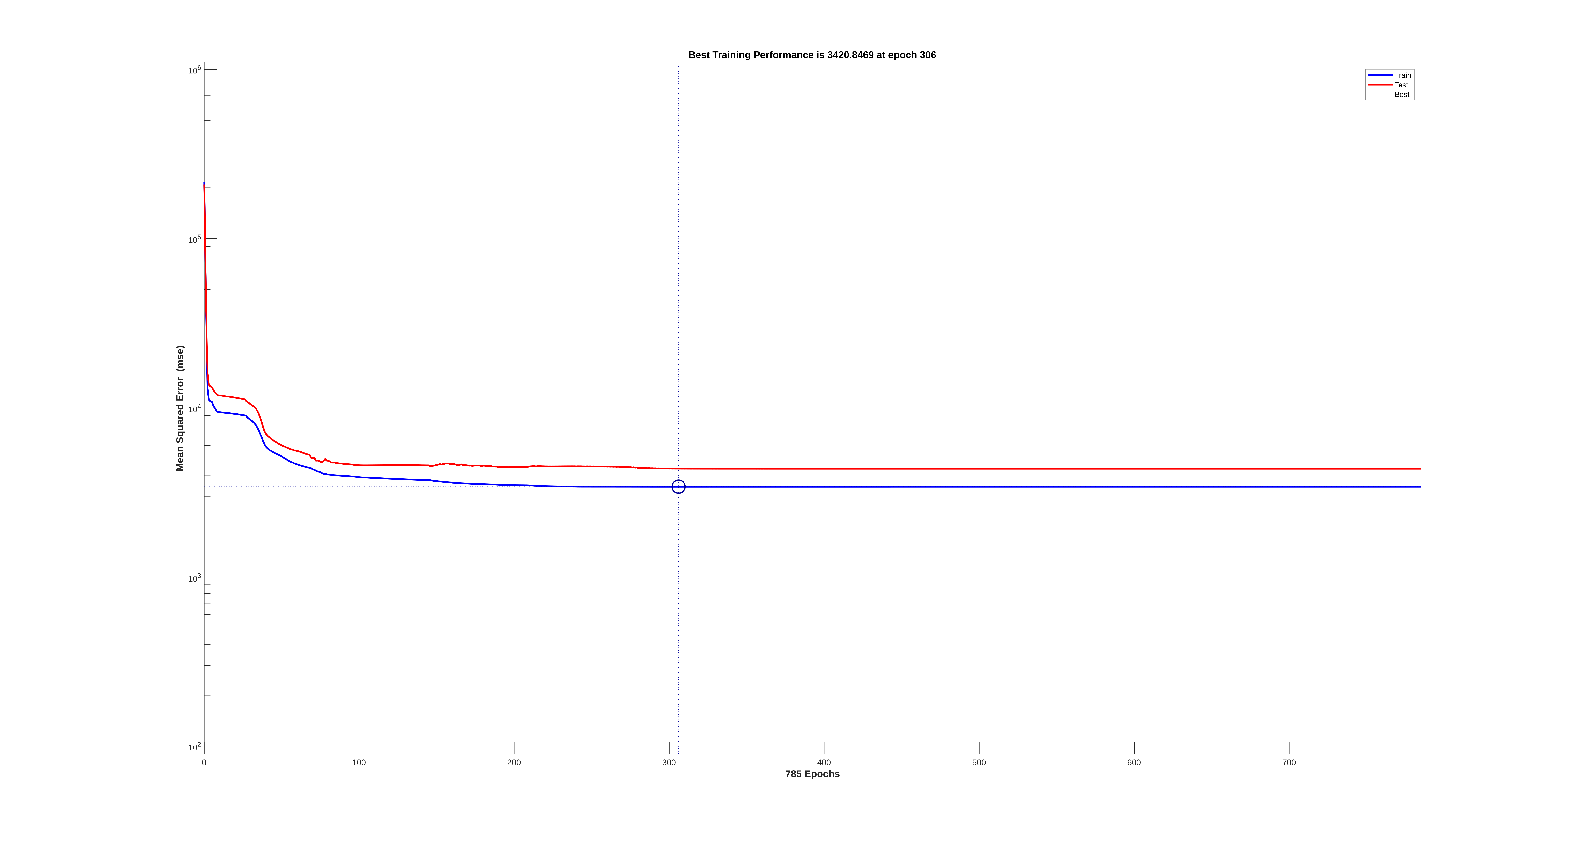
\includegraphics[width=\textwidth, trim=2.95cm 1.1cm 2cm 0.8cm,
		clip]{mlpmeantrainperformance}
		\caption{Training performance plot for the ECG's mean
		estimation network.}\label{fig:mlpmeantrainperformance}
	\end{subfigure}
	\begin{subfigure}{\textwidth}
		\centering
		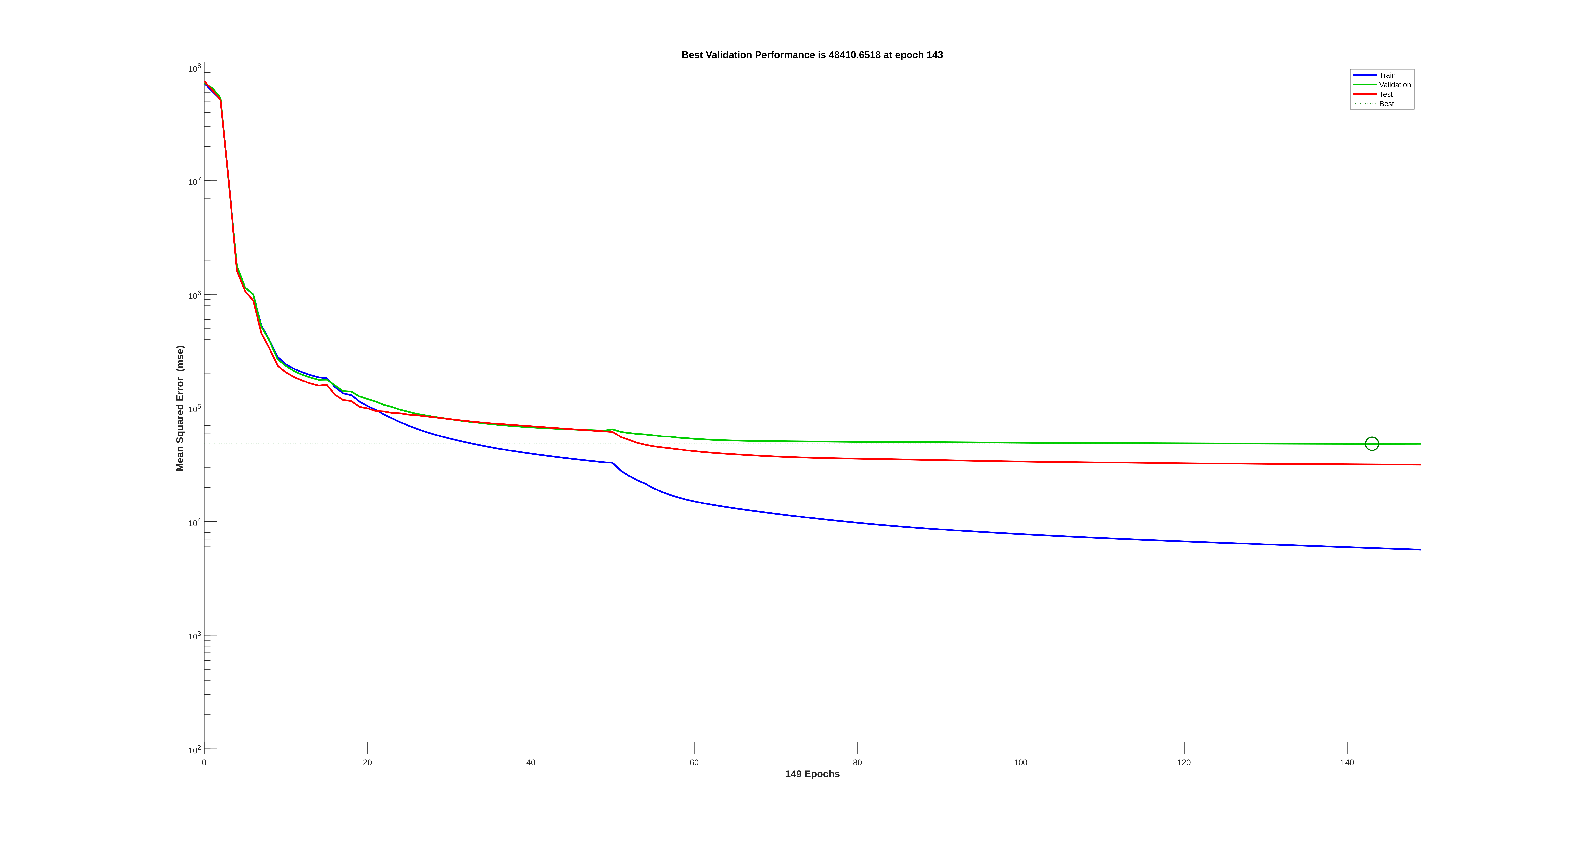
\includegraphics[width=\textwidth, trim=2.95cm 1.1cm 2cm 0.8cm,
		clip]{mlpstdtrainperformance}
		\caption{Training performance plot for the ECG's standard
		deviation estimation network.}\label{fig:mlpstdtrainperformance}
	\end{subfigure}
	\caption{Training performance plots for the two
	networks.}\label{fig:mlptrainperformance}
\end{figure}

\vfigref{fig:mlpstdregression} shows the regression plot for the ECG's standard
deviation estimation network. The network performs very well, with a
coefficient \(R = 0.99184\) for the test set and \(R = 0.99616\) for the entire
dataset.

\begin{figure}[htbp]
	\centering
	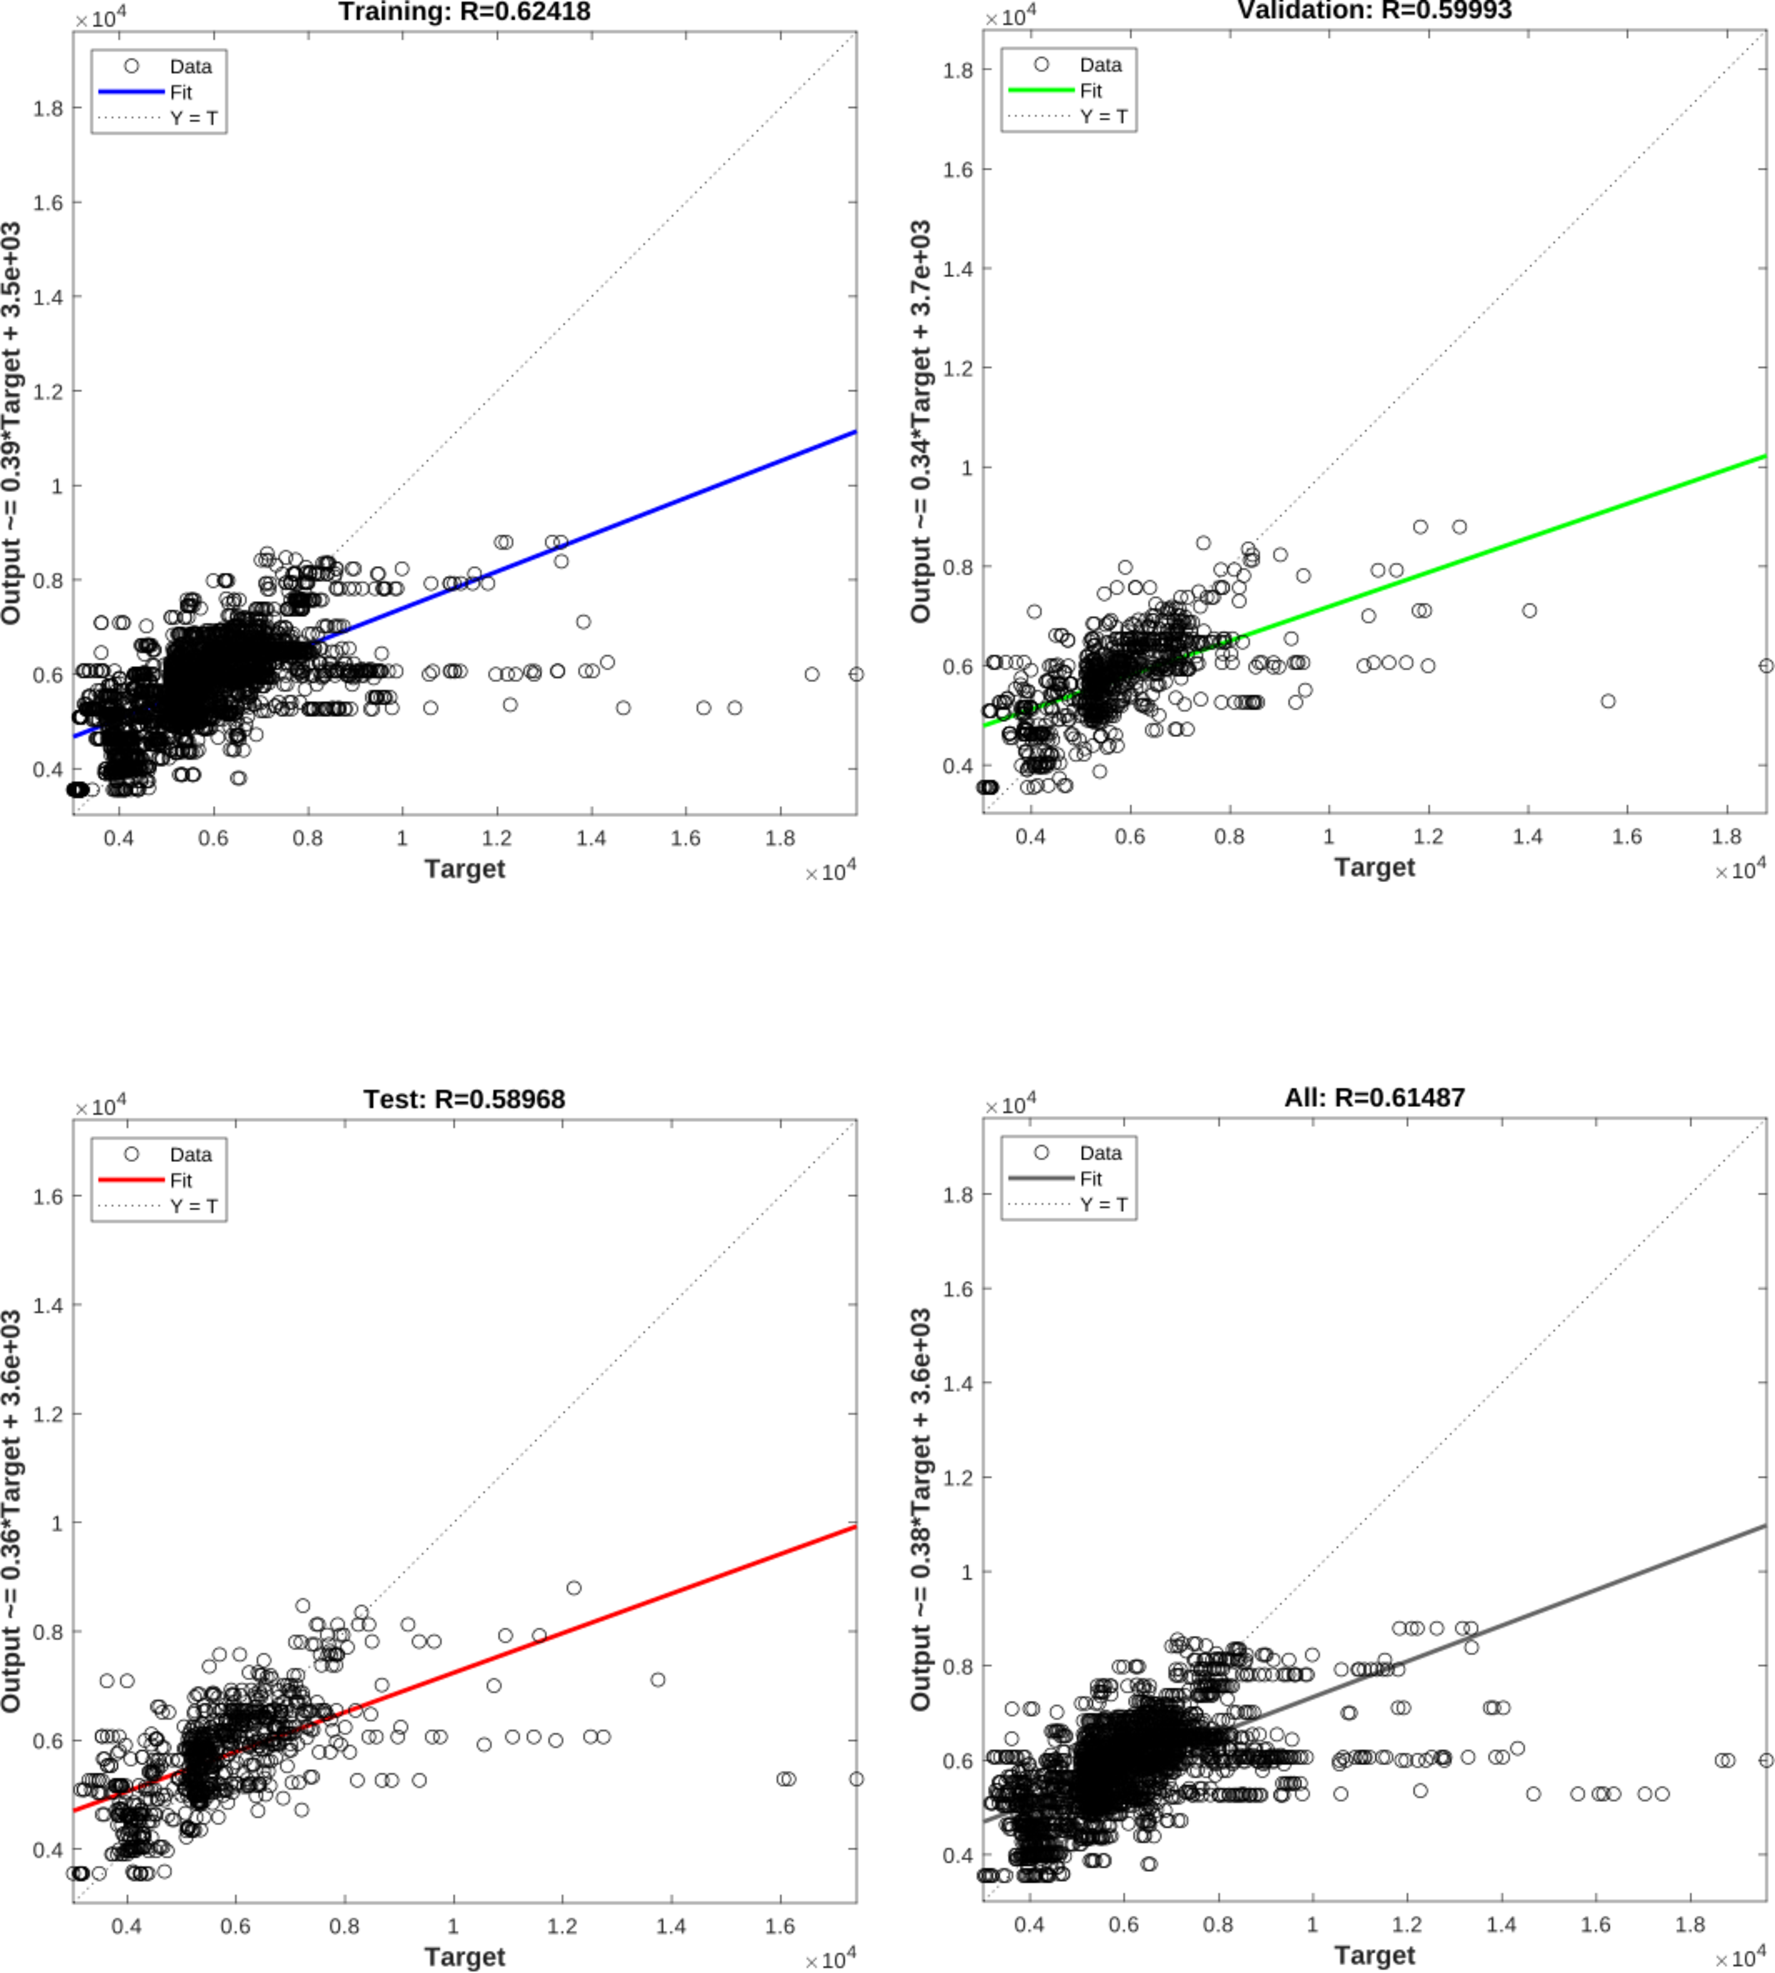
\includegraphics[width=\textwidth]{mlpstdregression}
	\caption{The regression plot for the ECG's standard deviation
	estimation network shows excellent
	results.}\label{fig:mlpstdregression}
\end{figure}

The ECG's mean estimation network performances are not so good (but still
valuable), as shown in \vfigref{fig:mlpmeanregression}: we have \(R = 0.85045\)
for the test set and \(R = 0.85761\) for the entire dataset. This latter
network will be the subject of \chref{ch:cnn}.

\begin{figure}[htbp]
	\centering
	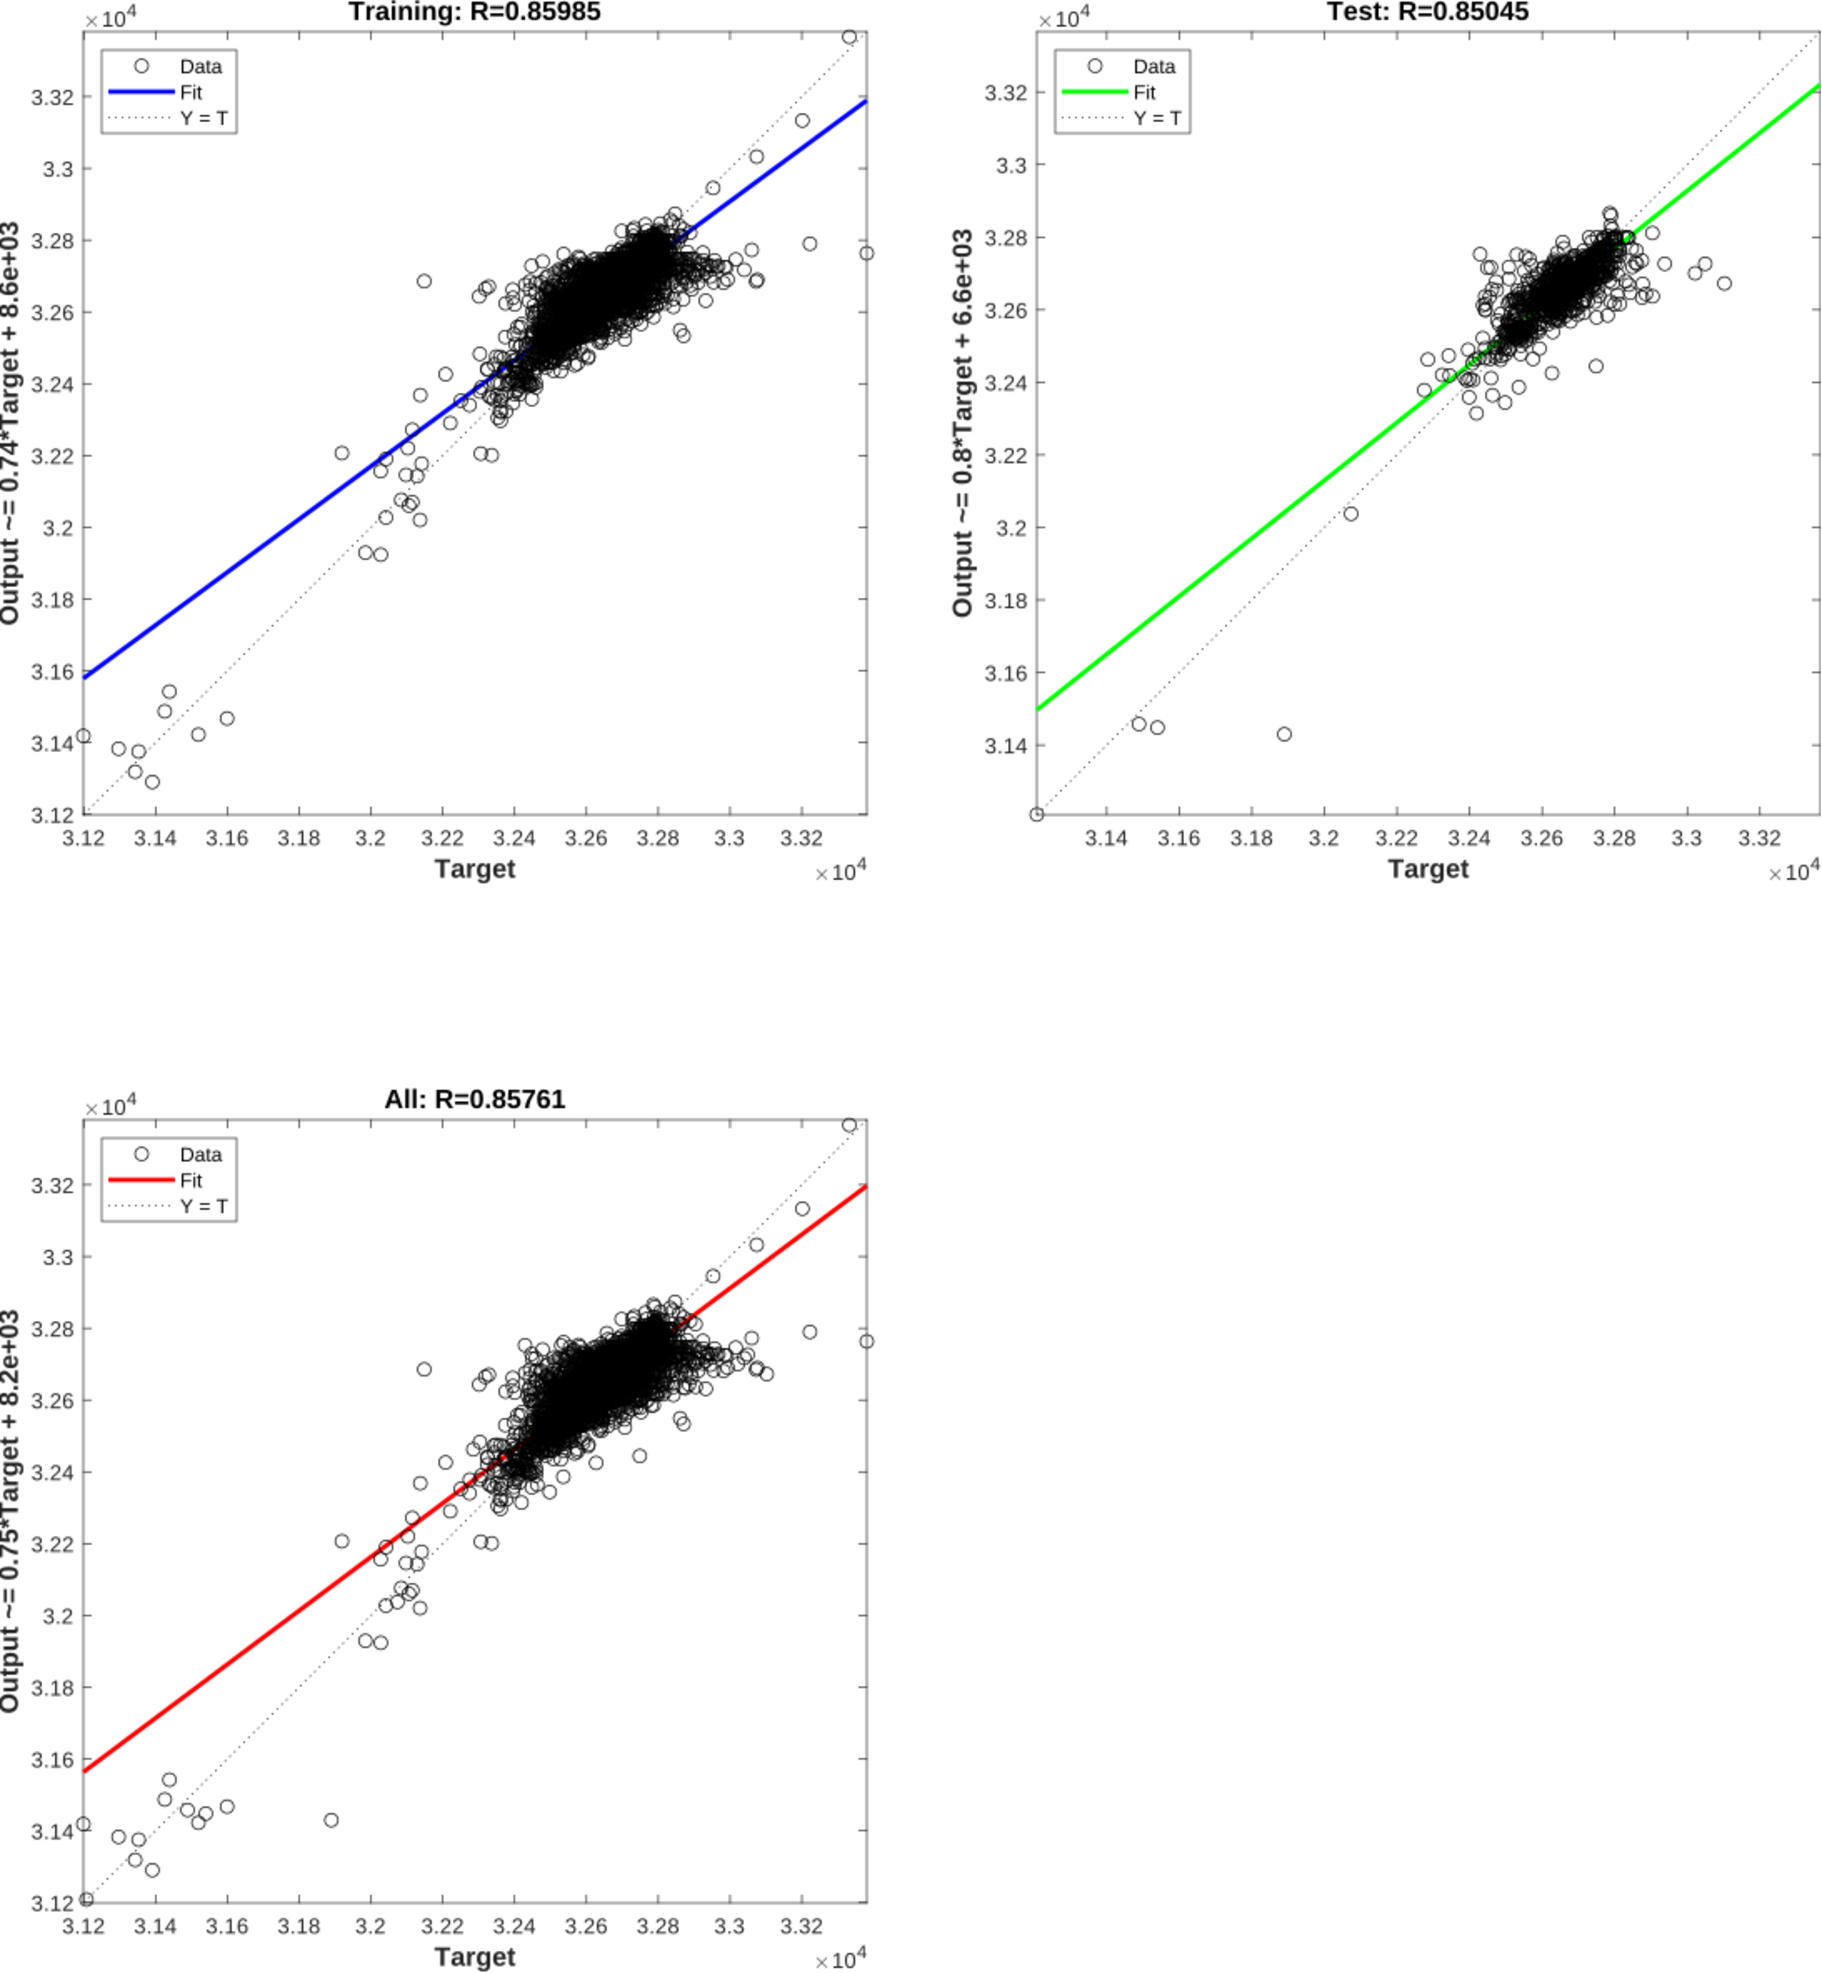
\includegraphics[width=\textwidth]{mlpmeanregression}
	\caption{The regression plot for the ECG's mean estimation network
	shows good, but not excellent, results.}\label{fig:mlpmeanregression}
\end{figure}

\vfigref{fig:mlperrorhists} shows the error histograms for both networks.

\begin{figure}[htbp]
	\centering
	\begin{subfigure}{\textwidth}
		\centering
		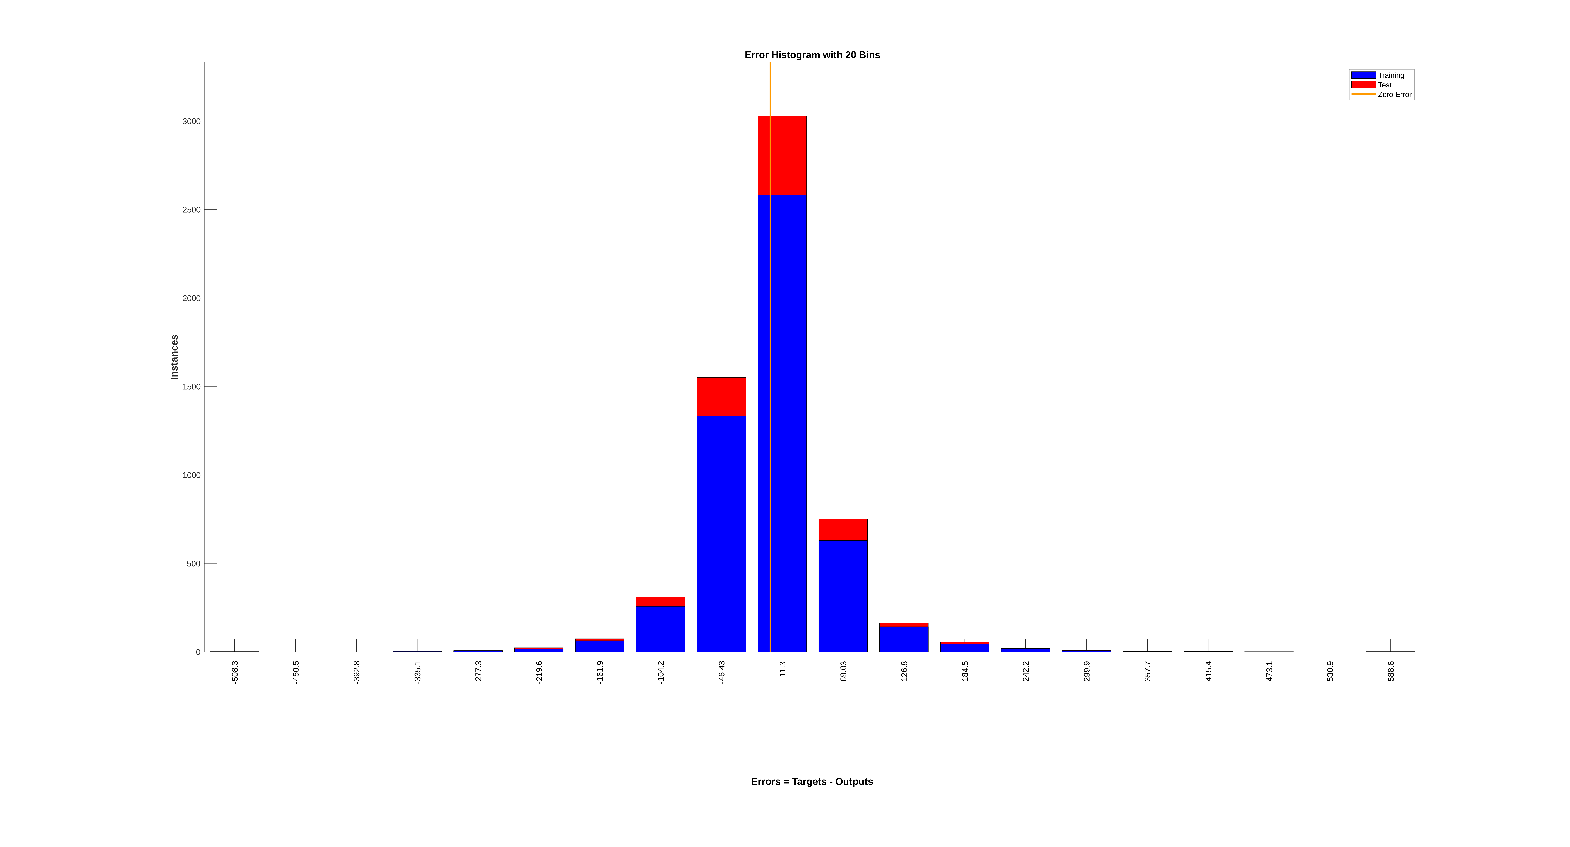
\includegraphics[width=\textwidth, trim=2.9cm 1cm 2cm 0.8cm,
		clip]{mlpmeanerrorhist}
		\caption{Error histogram for the ECG's mean estimation
		network.}\label{fig:mlpmeanerrorhist}
	\end{subfigure}
	\begin{subfigure}{\textwidth}
		\centering
		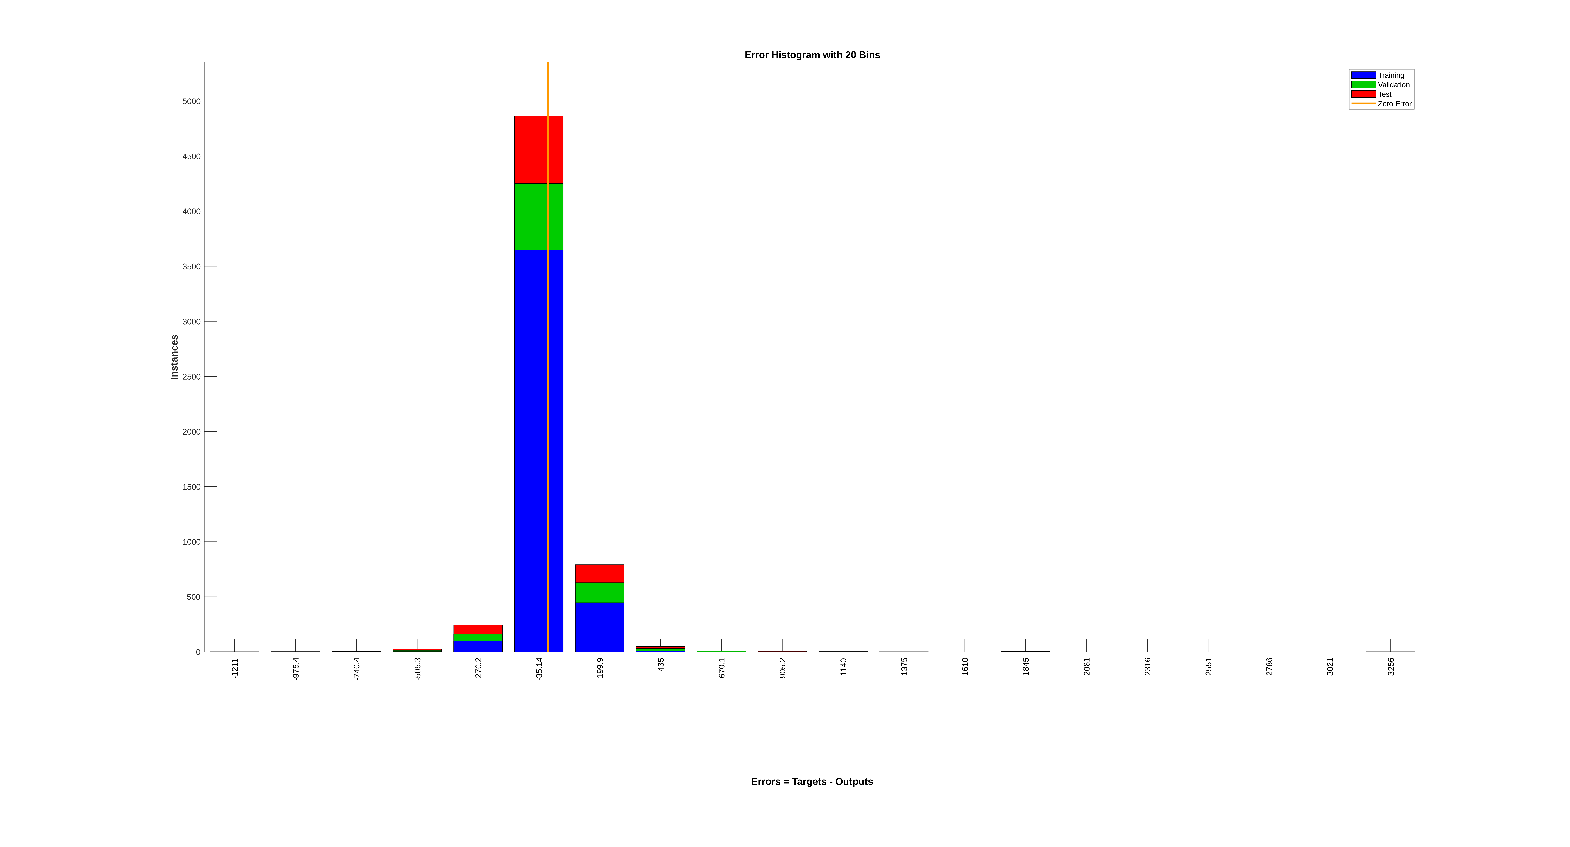
\includegraphics[width=\textwidth, trim=2.9cm 1cm 2cm 0.8cm,
		clip]{mlpstderrorhist}
		\caption{Error histogram for the ECG's standard deviation
		estimation network.}\label{fig:mlpstderrorhist}
	\end{subfigure}
	\caption{Error histograms for the two
	networks.}\label{fig:mlperrorhists}
\end{figure}

\section{Final Long Short-Term Memory Recurrent Neural
Network}\label{sec:rnnfinalrnn}

The final RNN is shown in \lstref{lst:finalrnn}.

\lstinputlisting[language={matlab}, label={lst:finalrnn},
style={Matlab-editor}, basicstyle={\footnotesize\ttfamily}, caption={The final
RNN architecture and training options.}]{rnndef.m}

This network has been trained for \(350\) epochs. Training ended after
\(33337\) iterations (\(238\) epochs plus some iterations), due to validation
loss not improving anymore. The network achieved excellent results with \(R >
0.99\) for all sets. Complete results are shown in \lstref{lst:rnnresults}.
\figref{fig:rnnregression} shows the regression plots for the RNN.
\figref{fig:rnnpredictions} shows an example of how the RNN predicts values for
the ECG.

\lstinputlisting[language={}, label={lst:rnnresults},
caption={Results of the final Long Short-Term Memory Recurrent Neural
Network.}]{rnnresults.txt}

\begin{figure}[htbp]
	\centering
	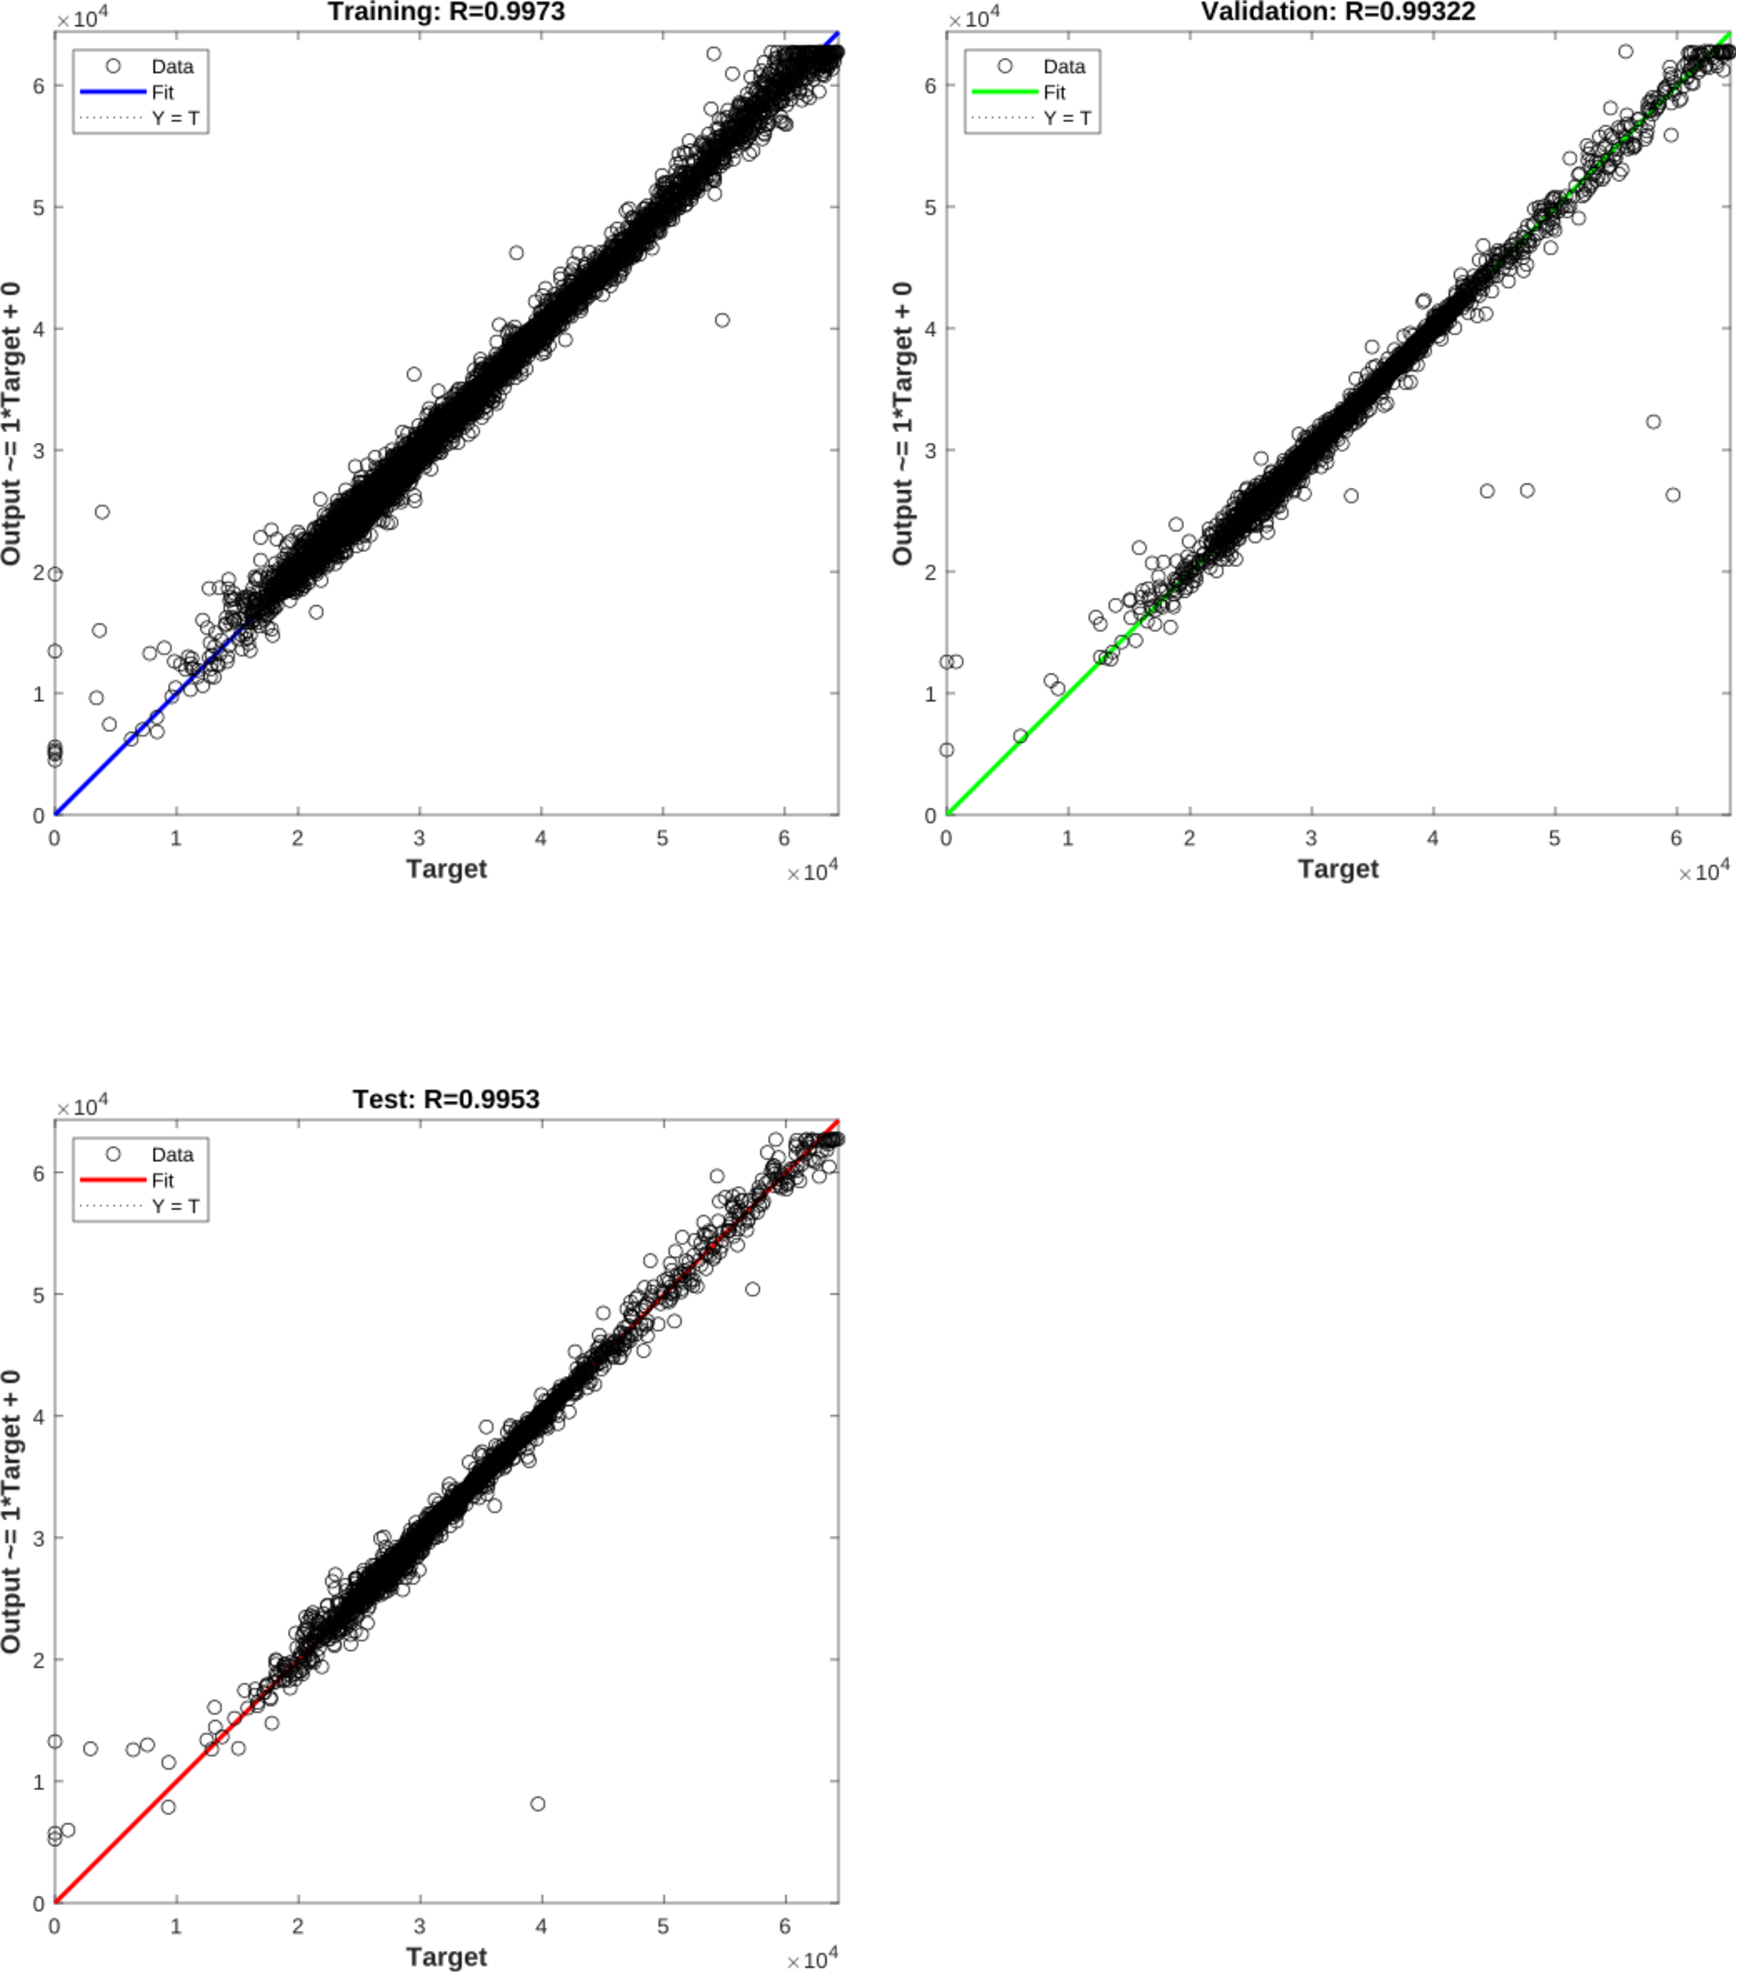
\includegraphics[width=\textwidth]{rnnregression}
	\caption{Regression plots for all three sets for the LSTM RNN
	that predicts values for the ECG.}\label{fig:rnnregression}
\end{figure}

\begin{figure}[htbp]
	\centering
	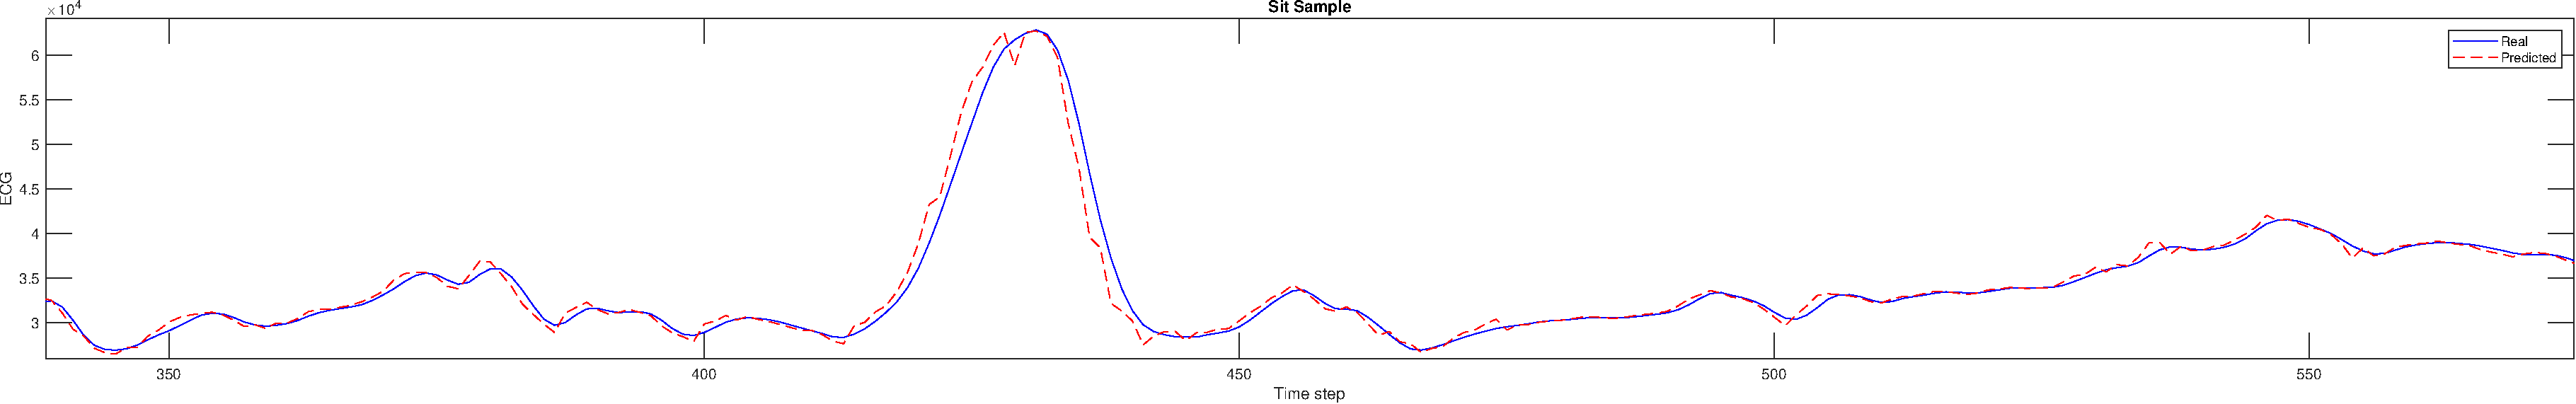
\includegraphics[width=\textwidth]{rnnpredictions}
	\caption{The 2 lines nearly overlap each other, proving that the RNN
	performs very well (zoom: this is vector
	graphics).}\label{fig:rnnpredictions}
\end{figure}

